% The body of every paper in this folder: long sections of text, inline and display math, a list, a listing, three
% figures and two tables in the middle sections, a footnote, and references. Each paper sets the type of the
% captions, the tables, the listing, the figure labels, and two sections with \sizeofcaptions,
% \sizeoftables, \sizeoflisting, \sizeoffigures, and \sizeofsections.
\section{Introduction}
Developers who work on the same files in parallel branches must resolve the conflicts that a merge reports. Each
conflict stops the integration of the change until a developer edits the conflicting lines by hand. This paper
presents a predictor that ranks the files of a pull request by the chance that a merge will report a conflict in
the file, before any developer merges the branch.
\lipsum[1-8]

\section{Background}
{\sizeofsections\lipsum[9-14]\par}
\begin{itemize}
\item A textual conflict arises when two branches edit the same lines of a file.
\item A build conflict arises when the merged code fails to compile although each branch compiles.
\item A test conflict arises when the merged code fails a test that each branch passes.
\end{itemize}
\lipsum[15-18]

\section{Approach}
\begin{figure}[t]
\centering
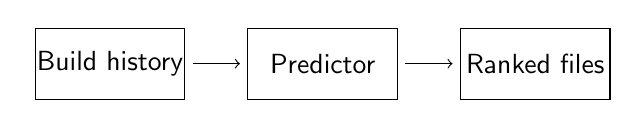
\begin{tikzpicture}[every node/.style={font=\sffamily\sizeoffigures}]
\draw (0,0) rectangle (1.9,0.9) node[midway] {Build history};
\draw[->] (2.0,0.45) -- (2.6,0.45);
\draw (2.7,0) rectangle (4.6,0.9) node[midway] {Predictor};
\draw[->] (4.7,0.45) -- (5.3,0.45);
\draw (5.4,0) rectangle (7.3,0.9) node[midway] {Ranked files};
\end{tikzpicture}
\caption{\sizeofcaptions The predictor reads the build history of a project and ranks the files of each pull request
by the chance of a merge conflict.}
\label{fig:overview}
\end{figure}
For a file $f$ of a pull request $p$, the predictor computes the change distance $d(f, p)$ as the number of lines
between the edits of the two branches and the conflict score
\begin{equation}
s(f, p) = b_0 + b_1 d(f, p) + b_2 h(f),
\end{equation}
where $h(f)$ counts the earlier conflicts of the file over the last $n$ merges.
\lipsum[19-22]
\begin{lstlisting}[language=Java,basicstyle=\ttfamily\sizeoflisting]
double score(FileChange change, History history) {
    double distance = change.lineDistance();
    double earlier = history.conflictsOf(change);
    return b0 + b1 * distance + b2 * earlier;
}
\end{lstlisting}
\lipsum[23-25]

\section{Evaluation}
\begin{table}[t]
\caption{\sizeofcaptions Projects of the evaluation}
\label{tab:projects}
\centering
\sizeoftables
\begin{tabular}{lrrr}
\toprule
Project & Pull requests & Files & Conflicting files \\
\midrule
commons-lang & 212 & 1,904 & 61 \\
guava & 188 & 2,311 & 49 \\
jackson-core & 141 & 1,077 & 38 \\
junit5 & 176 & 1,688 & 44 \\
mockito & 133 & 902 & 27 \\
spring-boot & 241 & 3,402 & 72 \\
\midrule
Total & 1,091 & 11,284 & 291 \\
\bottomrule
\end{tabular}
\end{table}
\begin{figure}[t]
\centering
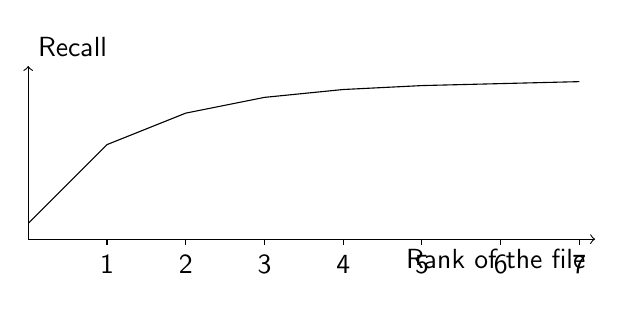
\begin{tikzpicture}[every node/.style={font=\sffamily\sizeoffigures}]
\draw[->] (0,0) -- (7.2,0) node[below left] {Rank of the file};
\draw[->] (0,0) -- (0,2.2) node[above right] {Recall};
\draw (0,0.2) -- (1,1.2) -- (2,1.6) -- (3,1.8) -- (4,1.9) -- (5,1.95) -- (7,2.0);
\foreach \x in {1,...,7} \draw (\x,0) -- (\x,-0.08) node[below] {\x};
\end{tikzpicture}
\caption{\sizeofcaptions Recall of the predictor at each rank over the 1,840 pull requests.}
\label{fig:recall}
\end{figure}
\lipsum[26-30]\footnote{The predictor and its data are available to the reviewers.}
\begin{table}[t]
\caption{\sizeofcaptions Conflicting files found at each rank}
\label{tab:recall}
\centering
\sizeoftables
\begin{tabular}{lrrrr}
\toprule
Rank & Found & Missed & Recall & Precision \\
\midrule
1 & 287 & 216 & 57.1 & 68.2 \\
3 & 371 & 132 & 73.8 & 51.6 \\
5 & 412 & 91 & 81.9 & 42.0 \\
10 & 455 & 48 & 90.5 & 27.3 \\
\bottomrule
\end{tabular}
\end{table}
\begin{figure}[t]
\centering
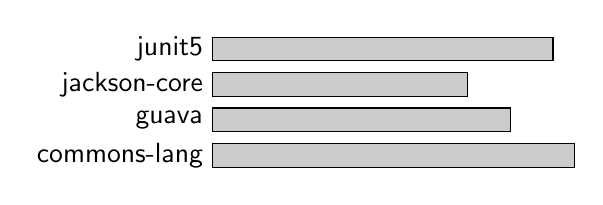
\begin{tikzpicture}[every node/.style={font=\sffamily\sizeoffigures}]
\foreach \y/\name/\len in {0/commons-lang/5.1, 0.45/guava/4.2, 0.9/jackson-core/3.6, 1.35/junit5/4.8} {
\draw[fill=gray!40] (1.8,\y) rectangle (1.8+\len*0.9,\y+0.3);
\node[left] at (1.8,\y+0.15) {\name};
}
\end{tikzpicture}
\caption{\sizeofcaptions Median time to resolve a conflict in each project, in hours.}
\label{fig:time}
\end{figure}
\lipsum[31-36]

\section{Related Work}
{\sizeofsections\lipsum[37-48]\par}

\section{Conclusion}
\lipsum[49-54]

\begin{thebibliography}{9}
\bibitem{a} A. Author and B. Author, ``A study of merge conflicts,'' in \emph{Proc. Conf.}, 2020, pp. 1--10.
\bibitem{b} C. Author, ``Build conflicts in Java projects,'' \emph{J. Softw.}, vol. 3, no. 2, pp. 11--20, 2021.
\bibitem{c} D. Author, E. Author, and F. Author, ``Predicting conflicts from change histories,'' in
\emph{Proc. Conf.}, 2022, pp. 21--30.
\bibitem{d} G. Author, ``Proactive detection of merge conflicts,'' \emph{J. Softw.}, vol. 5, no. 1, pp. 1--15,
2023.
\end{thebibliography}
